%%%%%%%%%%%%%%%%%%%%%%%%%%%%%%%%%%%%%%%%%%%%%%%%%%%%%%%%%%%
\section{Theory}
\label{sec:theory}
%%%%%%%%%%%%%%%%%%%%%%%%%%%%%%%%%%%%%%%%%%%%%%%%%%%%%%%%%%%
This section examines the problem of mapping with uniform inputs in 1 and 2 dimensions.
 
\subsection{Mapping in 1D}
We begin with the single particle case, then proceed to the $n$ particle case.

\subsubsection{1D mapping with 1 particle}
A particle initialized uniformly randomly in a linear free-space $m$ units wide.  To map this region the particle needs to choose one direction, move until it hits a boundary, and then switch direction and move until it reaches the other boundary.


Without loss of generality, assume the particle always starts going left, and label the free-space from 1 to $m$ left to right.  If the initial position is 1, the particle tries to move 1 unit to the left, but is stopped by the boundary. The particle then moves $m-1$ moves to the right.  The final $m$th move right results in a collision with the right wall, and thus mapping requires $m+1$ moves. This is the minimum number of moves.  The worst case is if the particle starts at $m$, requiring $2m$ moves: $m$ moves to the left and $m$ moves to the right.

\begin{figure}
\begin{center}
	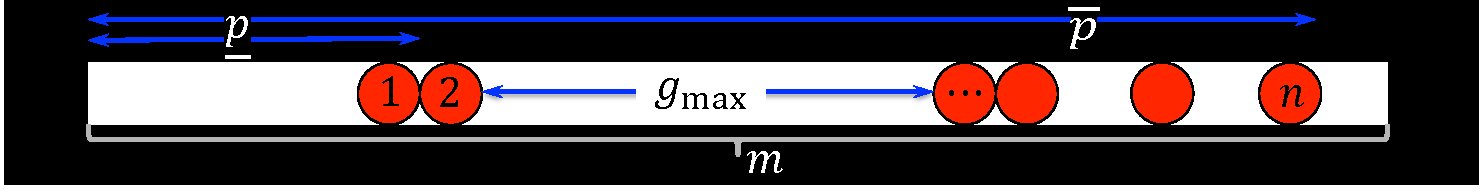
\includegraphics[width=1.0\columnwidth]{MaxGapm20n5s1v3.pdf}
\end{center}
\caption{\label{fig:coverage1d}
Exploring a 1D environment of size $m$ with $n$ particles. Here $m=20$ and $n=6$. $\pmin=4$, $\pmax=1$ and $g_{max}= 7$
}
\end{figure}


The expected number of moves for one particle to cover a 1D area of length $m$ is 
\begin{align}
\frac{1}{m} \sum _{i=1}^m (i+m) &= \frac{3 m+1}{2}  \label{eq:expectedMoves1particle1D}
\end{align}

\subsubsection{1D mapping with n particles}

Let $\mathbf{p}$ be the list of positions of $n$ particles uniformly distributed from $[1, m]$.
As shown in Fig. \ref{fig:coverage1d}, the number of moves to discover the left and right boundaries is bounded by the maximum and minimum particles $ \pmin =\min(\mathbf{p})$, $\pmax =\max(\mathbf{p})$, requiring moving left $\pmin$, followed by a move of $m-(\pmax - \pmin ) $ right.
When $n=m$, the algorithm requires 2 moves, one left, one right.
The minimum time with $n\in[2,m-1]$ occurs with $\pmin$ at 1 and the $\pmax$ at $m$, requiring 3 moves, 1 left followed by 2 moves to the right.  

The maximum $2(m-n+1)$ occurs when the particles are arranged from $m-n$ to $m$, requiring $m-n+1$ moves to the left, followed by $m-n+1$ moves to the right.

This is drawing without replacement $n$ times from the set $[1, m]$.  The minimum is distributed between 1 and $m-n$, the maximum is distributed between $n$ and $m$.

The expected number of moves to reach both boundaries for $n$ particles in 1D is 
\begin{align}
\frac{1}{{m \choose n}} \sum_{\pmin = 1}^{m-n+1}  \sum_{\pmax = \pmin +n-1}^{m}   {\pmax -\pmin-1 \choose n-2} \left( 2 \pmin +m- \pmax +1\right)  \nonumber \\
= \frac{3(1+m)}{1+n}\label{eq:expectedMoveskparticles1D}
\end{align}

To fully \emph{cover} the area from 1 to $m$ requires that every position from 1 to $m$ be visited by at least one particle.  This time is dominated by the maximum gap $\overline{g}$. The total number of moves is then $ 2 \pmin +m- \pmax +1 + \max \left( \overline{g} - \left(\pmin + m-\pmax \right),0 \right)$.


 If all the particles are unit size, there are $m-n$ spaces, and these can be located before, between, or after the $n$ particles in $n+1$ locations giving ${m-n \choose n+1}$ possible configurations. The largest gap can be calculated exactly using a recurrence equation \cite{reviriego2011expected}, but a tight bound when
$m>n \log{n}$ is $\frac{m-n}{n+1} + \Theta \left( \sqrt{\frac{ (m-n)\log(n+1)}{n+1}} \right)$\cite{Raab1998}. 

%\todo{I want an analytical result for the expected maximum gap. An analytical result for the maximum gap is given in \url{http://www.nebrija.es/~jmaestro/esa/papers/JDA2011.pdf}, but I have been unable to solve the coefficients in equation (18).  The same result is also in Section 9.4 of An Introduction to the Analysis of Algorithms, Second Edition by Robert Sedgewick and Philippe Flajolet, which I have ordered but don't have yet. -Aaron}
%Define the probability of any given combination $T= {m \choose n}^{-1}$.  
%If $n+1 = m$ there is one gap of size $1$, and $n+1$ possible locations.
%The maximum gap size is $m-n$, and this gap can be placed before or after any of the $n$  numbers, for a total of $n+1$ possible positions.


\subsubsection{1D mapping with scan and move costs}
 Often scanning (imaging) and moving the particles costs time and energy.
 When controlling particles with MRI as in \cite{chanu2008adapting}, the MRI machine iterates between imaging and applying gradient forces to move the particles.
 This section examines 1D mapping when scanning the workspace and moving the particles a unit distance have associated costs. 
The objective is to minimize a linear comination of costs for moving and measuring; however, the precise respective coefficients may be subject
to change, or even unknown in advance turning this into a {\em bicriteria problem}, in which both parameters need to be within 
a bounded rato of those in an optimal solution. For simpler notation, we write $(a,b)$ for a schedule that involves $a$ unit steps and $b$ scans.

For a more details analysis, assume that the left boundary is located $D$ units to the left of the leftmost particle.
(This analysis can be applied in both directions.)
The theoretically optimal, yet elusive, solution requires scanning the workspace to map particle locations,
moving $D+1$ units to the left, 
then scanning to detect that the leftmost particle has only moved $D$ units and thus has encountered the wall,
for a total cost of $(D+1,2)$ for the schedule.

We can achieve a schedule with $D+1$ steps by scanning after each step, for a total cost of $(D+1,D+2)$;
while this is optimal with respect to steps, the involved scan cost is large compared to the optimum.
At the expense of increasing the number of can reduce the number of scans by successively doubling the number 
of steps between scans, i.e., performing the $i$th scan after $2^i$ steps, resulting in total cost at most $(2D+2,\log D)$; replacing
the base of $2$ by an arbitrary constant $k$, we get $(k\times(D+1), \log_k D)$. This is within a constant of the optimal 
On the other hand, moving a sufficiently large number $M$ of steps (known to satisfy $M\geq D$) before performing the second 
scan yields $(M,2)$, which is optimal with respect to scan cost, but bad in terms of the cost for motion.

Balacing the competitive factor for both parameters can be achieved as follows:
perform the $i$th scan at position $i^i$. As it turns out, this yields a simultaneous competitive factor of 
$O(\log D/\log\log D)$ for {\em both} parameters.

\begin{theorem}
\label{th:eyetoeye}
The hyperexponential search sequence $i^i$ yields an simultaneous competitive factor of $O(\log D/\log\log D)$ for {\em both} parameters
of the bicriteria search problem; this is best possible.
\end{theorem}

\begin{proof}
Let us first consider the number of scans.
If the boundary is properly detected in step $j+1$, the particle must have encountered it between steps $j$ and $j+1$, i.e. $j^j \leq D < (j+1)^{j+1}$.
Now we can employ the Lambert $W$ function, which is the inverse function of $f(x)=xe^x$; note that 
$$\log x = W(\log x)*e^{W(\log x)},$$ 
so
	$$\log \log x = (\log W(\log x) + W(\log x)),$$
and therefore
	$$W(\log x) \in \Theta(\log \log x).$$

This implies that $j\leq \log D/ W(\log D)$ (the inverse of $j^j$), hence $\Theta(\log D/ \log\log D)+1$ scans have been made, while the optimum are $2$ scans.

The moved distance is $(j+1)^{j+1}$, while the optimum is $D\geq j^j$.
Hence, we get the ratio 
\begin{align}
\frac{(j+1)^{(j+1)}}{j^j}=(j+1)\frac{(j+1)^j}{j^j},\label{eq:MoveDistanceRatio}
\end{align}
 where $0\leq \frac{(j+1)^j}{j^j}\leq \mathrm{e}$ for $j>0$.
 
Because $j\leq \log D/ W(\log D)$, we obtain 
\begin{align}
\frac{(j+1)^{(j+1)}}{j^j}\leq \mathrm{e}\frac{log n}{ W(\log n)}+\mathrm{e}\label{eq:MoveDistanceRatioInequality}
\end{align}
 for $j>0$. Clearly, this is again in within a factor of $\Theta(\log D/ \log\log D)+1$ of the optimum.
\end{proof}

%\subsubsection{German tank problem}
%With multiple samples it is now possible to guess which direction is closer to the edge?  The population maximum is 
%uniformly minimum-variance unbiased estimator "The sample maximum plus the average gap between observations in the sample" --> but this will give the same distance to each side.  

\subsection{Mapping in 2D}


\subsubsection{2D mapping with 1 particle}
The shortest path for mapping with 1 particle is a version of depth-first search that halts when all boundaries have been reached.
As long as the freespace is connected, DFS is the optimal solution to mapping.
%\todo{Q2.Domink --- Prove that DFS is the optimal solution with 1 particle }
%<Dominik> <- this tag is just to ease possible merges. Feel free to edit or delete.
Even if the environment is known in advance, the problem is NP-hard as can be shown by a trivial reduction to Hamiltonian Paths in Grid Graphs \cite{itai1982hamilton}. %NP-hardness shown in Itai, Alon, Christos H. Papadimitriou, and Jayme Luiz Szwarcfiter. "Hamilton paths in grid graphs." SIAM Journal on Computing 11.4 (1982): 676-686.
One can easily show that a simple depth-first-search guarantees an optimal ratio of $2$: the depth-first tree has $m-1$ edges and each edge is traversed at most twice. 
Any path that covers $m$ fields needs to traverse least $m-1$ edges, the depth-first-search hence is at most twice as long as an optimal coverage path.

For showing that no algorithm can perform better one needs only a simple 1-dimensional graph that goes to the left and to the right.
If the algorithm chooses to go arbitrarily to one side, we can make it do a long walk of length $m$ and then return it just for a single field on the other side ($2*m+1$ vs $2+m$).
If the algorithm decides to switch the direction after some time after arbitrary zig-zags (of increasing cost) of cost $z$ (center to one side to other side) we decide that there is a single field on both sides.
The algorithm now needs to go one additional time from one side to the other and back (cost $>z$) while the optimum cost would have been $\leq z+3$.
If the algorithm switches from the second form to the first, the first argument still applies.

%TOURS (related work, actually doesn't belong here but you probably find it here most easily. Just to help with related work.):
Most previous work on grid graph exploration focused on exploration tours, i.e., after exploration one has to go back to the start position.
If the environment is known in advance, this equals the traveling salesman problem and a PTAS is known~\cite{klein2008linear}. % Philip N. Klein.  A linear-time approximation scheme for TSP in undirected  planar  graphs  with  edge-weights.  SIAM  Journal  on  Computing , 37(6):1926–1952, 2008.
If the environment is unknown, as it is in our case, the best achievable competitive ratio is $2$ in general grid graphs (achieved by depth first search) and $7/6$ for simple grid graphs ($4/3$ achieved by smartDFS \cite{icking2005exploring}). %Icking et al. http://link.springer.com/chapter/10.1007/11533719_53 http://www.geometrylab.de/applet-55
%</Dominik>

\subsubsection{2D mapping with n particles}

The problem with mapping with $n$ particles is also to identify which move sequence guarantees the shortest path in the worst case.
 For each particle, at the beginning there can be at most four frontiers to be explored. As the particles begin to move, the number of frontier cells explored and the number of free cells identified increases. 
 If we implement a random move algorithm as described in Alg.~ \ref{alg:randommove}, at each step the particles all move in the same randomly selected direction until there are no Frontier cells left on the map. 
 $MoveType$ is a vector that holds the four possible move types. 
 The map $\mathbf{M}$ is a matrix the size of the work space. 
 Each cell of  $\mathbf{M}$ holds one of five values that denote: $Particle$, $Frontier$, $Unknown$, $Free space$ and $Obstacle$. 
 At each step {\sc Frontier} returns the locations of frontier nodes in $\mathbf{M}$ and $\mathbf{r}$ has the list of particle locations.
 The $move$ is implemented to update the map $\mathbf{M}$ and the particle locations $\mathbf{r}$ by calling {\sc Move\&\!Update}. 
 This method requires minimal computation and is probabilistically complete, so eventually the swarm maps the free space~\cite{kahn1989cover}. 
 However, this method of mapping is inefficient, resulting in long mapping times,  especially with small numbers of particles in large, torturous freespaces. 

  \begin{algorithm}
\caption{\sc RandomMoves($\mathbf{M},\mathbf{r}$)   \label{alg:randommove}}
\begin{algorithmic}[1]
\State$MoveType = \{r,l,u,d\}$ 
\While{$|${\sc Frontier}$(\mathbf{M})| >0  $}
%\While{ $|\mathbf{M}.FrontierNodes| >0  $}
\State$move \gets$ {\sc random}$(MoveType)$
\State $\{\mathbf{M}, \mathbf{r}\} \gets ${\sc Move\&\!Update}$(move, \mathbf{M}, \mathbf{r}) $
\EndWhile
\end{algorithmic}
\end{algorithm}

A better way to map the world would be to move particles towards unexplored nodes. We could choose one particle as a lead particle and base all motion on the location of that particle. 
In Alg.~ \ref{alg:ElectParticle}, one of the particles is selected as the leader. 
As long as the number of frontiers to be visited is atleast one, the algorithm proceeds by generating a $moveSeq$ from the current position of the elect particle to the nearest frontier node. 
The $moveSeq$ is generated by a {\sc Dijkstra} shortest path algorithm to which we feed the map $\mathbf{M}$, source $lead$, and the nodes {\sc Frontier}$(\mathbf{M})$. A representative $moveSeq$ is $\langle u,r,d,d,r,u,\ldots\rangle$. 
The list of moves in $moveSeq$ are implemented by iterativly calling the {\sc Move\&\!Update} function for the length of the list. 
This algorithm will surely explore the target frontier within the length of the list $moveSeq$. 
Every time {\sc Move\&\!Update} is implemented, the nearest frontier is updated and $moveSeq$ is also updated because as the particles start to move, the target frontier in each step might be explored by another particle which is not the elect particle. 
So, usually, with large swarm size it is possible that the whole $moveSeq$ need not be implemented. 
Only if the elect particle is the nearest particle to the target node, the complete $moveSeq$ is implemented. 
This is the case in Alg.~\ref{alg:ClosestFrontier} in which all the particles are considered and the $moveSeq$ is the list of moves required to move the swarm to it's closest frontier.  
  \begin{algorithm}
\caption{\sc ElectParticle($\mathbf{M},\mathbf{r}$)   \label{alg:ElectParticle}}
\begin{algorithmic}[1] 
\State $lead \gets$ {\sc random}$(\mathbf{r})$
\While{$|${\sc Frontier}$(\mathbf{M})| >0  $}
\State$moveSeq \gets$ {\sc Dijkstra}$(\mathbf{M},lead,${\sc Frontier}$(\mathbf{M}))$
\For {$iter:=1$ $\mathbf{ to}$ $|moveSeq| $ $\mathbf{ step }$ $ 1$} 
\State $\{\mathbf{M}, lead\} \gets ${\sc Move\&\!Update}$(moveSeq, \mathbf{M}, lead) $
 \EndFor
\EndWhile
\end{algorithmic}
\end{algorithm}

In Alg.~\ref{alg:ClosestFrontier} in each loop, all the moves in $moveSeq$ need to be implemented to explore the target frontier since it is the shortest possible route to a frontier cell. 
When the mapping is initiated, there will be 4$k$ equally valid destinations that can be visited since all four sides of each particle will be a frontier cell. 
The algorithm arbitrarily choose a direction to move to. 
Once frontiers are classified, there can be at most three more frontiers added per particle if it has landed on a free space or there will be a reduction of one frontier if the frontier cell contained an obstacle. 
Since each $moveSeq$ guarantees classification of one frontier node into obstacle or free space. If there are $n$ free spaces, the maximum possible frontier cells count will be $3(n-2)+6$. 
If for moveSeq generation left,up,right,down is the order of preference for direction of move in case of equidistant nodes, then as an example, for $k$ particles the maximum number of moves required to completely map the linear map environment will be 4($n$-$k$+1) if all the particles are arranged in adjacent cells on the right corner of the linear map. 
The simulation results in Section \ref{sec:simulation} show that both map complexity and distribution affect the number of moves taken to map the work space. In Alg.~\ref{alg:randommove} we used no information from the data except for checking completion. 
In Alg.~\ref{alg:ElectParticle} we use the location and distance data from one particle to map the work space. 
Finally in Alg.~\ref{alg:ClosestFrontier} we can push the performance of the mapping by utilizing all the data such as location of all particles and distance measurements from all frontiers. 

  \begin{algorithm}
\caption{\sc ClosestFrontier($\mathbf{M},\mathbf{r}$) \label{alg:ClosestFrontier}}
\begin{algorithmic}[1]
\While{$|${\sc Frontier}$(\mathbf{M})| >0  $}
\State$moveSeq \gets$ {\sc Dijkstra}$(\mathbf{M},\mathbf{r},${\sc Frontier}$(\mathbf{M}))$
\For {$iter:=1$ $\mathbf{ to}$ $|moveSeq| $ $\mathbf{ step }$ $ 1$}  
\State $\{\mathbf{M},\mathbf{r}\} \gets ${\sc Move\&\!Update}$(moveSeq, \mathbf{M}, \mathbf{r}) $

 \EndFor
  
\EndWhile
\end{algorithmic}
\end{algorithm}

\todo{Q7.Prove the greedy algorithm always works }

%\todo{insert plot of boundary nodes as a function of moves for 3 different values of no. of particles. n=100, n=500 and n=2000} 

Not sure how to do this.  We have experiments.  There are so many options for arranging the freespace.  

The minimum time is a rectangle $k$ units tall and $n/k$ wide, with the $n$ particles arranged along the left wall. 1 move left registers the left wall, repeating $n/k$ moves up and right to find the top boundary and the right boundary,  followed by $n/k -1$ moves down and left to find the bottom boundary, with one final move down to register the furthest left bottom boundary.  This is 4(n/k) moves. %1+2(N/K) + 2(N/k -1)+1 = 

%Better if particles are in a square with side $\sqrt{N}$ and are in a vertical column spaced $\sqrt{N}/k-1$ apart.  moving left, followed by moving

\todo{Q3.What is the worst case?  }

\todo{Q4.What is the complexity of the 2D problem?  }

\todo{Q5.Can we do better than the greedy algorithm for 2D coverage?  }

\todo{Q6.What is the running time for the greedy algorithm?  }


%\subsection{Mapping in 3D}

%\todo{We can do some experiments for this.  Perhaps draw wireframes for free spaces, draw red and blue cubes for unknown.  TODO: draw with red circles/spheres for particles.}





